\documentclass[tikz,border=2pt]{standalone}
\usepackage{amsmath}
\usepackage{pgfplots}
\pgfplotsset{compat=1.18}
\usetikzlibrary{arrows.meta}
\begin{document}
% Two solutions fixed by x_0, x_1 (orange). Left: roots 2, 3, x_0 = 1, x_1 = 4 give x_t = 2*3^t - 2^t
% = 1, 4, 14, 46. Right: roots +-i, x_0 = 1, x_1 = 0 give x_t = cos(pi t/2) = 1, 0, -1, 0, ... (period 4).
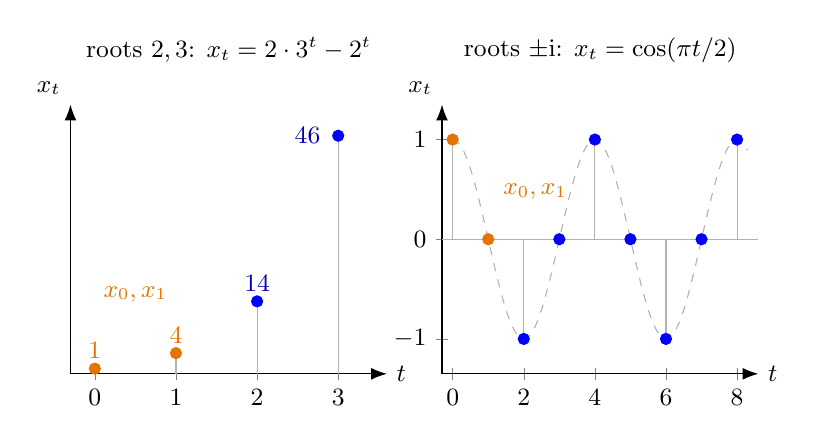
\begin{tikzpicture}[font=\small, >={Latex[length=2mm]}]
  \pgfplotsset{sd/.style={width=5.6cm, height=5cm, axis lines=left, axis line style={->},
      xlabel={$t$}, xlabel style={at={(1,0)}, anchor=west}, tick label style={font=\small},
      title style={font=\small, yshift=2mm}, clip=false}}
  \begin{axis}[sd, name=left, xmin=-0.3, xmax=3.6, ymin=0, ymax=52, xtick={0,1,2,3}, ytick=\empty,
      title={roots $2,3$: $x_t=2\cdot3^t-2^t$}]
    \addplot[gray!60, ycomb, thin] coordinates {(0,1) (1,4) (2,14) (3,46)};
    \addplot[only marks, mark=*, mark size=2pt, blue] coordinates {(2,14) (3,46)};
    \addplot[only marks, mark=*, mark size=2pt, orange!90!black] coordinates {(0,1) (1,4)};
    \node[orange!90!black, anchor=south] at (axis cs:0,1) {$1$};
    \node[orange!90!black, anchor=south] at (axis cs:1,4) {$4$};
    \node[blue!70!black, anchor=south] at (axis cs:2,14) {$14$};
    \node[blue!70!black, anchor=east] at (axis cs:2.9,46) {$46$};
    \node[orange!90!black, anchor=south] at (axis cs:0.5,12) {$x_0,x_1$};
    \node[anchor=south east] at (rel axis cs:0,1) {$x_t$};
  \end{axis}
  \begin{axis}[sd, at={(left.east)}, anchor=west, xshift=0.7cm, xmin=-0.3, xmax=8.6, ymin=-1.35, ymax=1.35,
      xtick={0,2,4,6,8}, ytick={-1,0,1}, 
      title={roots $\pm\mathrm{i}$: $x_t=\cos(\pi t/2)$}]
    \draw[gray!60, thin] (axis cs:-0.3,0) -- (axis cs:8.6,0);
    \addplot[gray!60, dashed, domain=0:8.3, samples=120] {cos(deg(pi*x/2))};
    \addplot[gray!60, ycomb, thin] coordinates {(2,-1) (4,1) (6,-1) (8,1)};
    \addplot[only marks, mark=*, mark size=2pt, blue] coordinates {(2,-1) (3,0) (4,1) (5,0) (6,-1) (7,0) (8,1)};
    \addplot[gray!60, ycomb, thin] coordinates {(0,1)};
    \addplot[only marks, mark=*, mark size=2pt, orange!90!black] coordinates {(0,1) (1,0)};
    \node[orange!90!black, anchor=south west] at (axis cs:1.15,0.3) {$x_0,x_1$};
    \node[anchor=south east] at (rel axis cs:0,1) {$x_t$};
  \end{axis}
\end{tikzpicture}
\end{document}
